\section{Common Gateway Interface (CGI)}
\ref{CGI}:
\begin{figure}[ht]
	\centerline{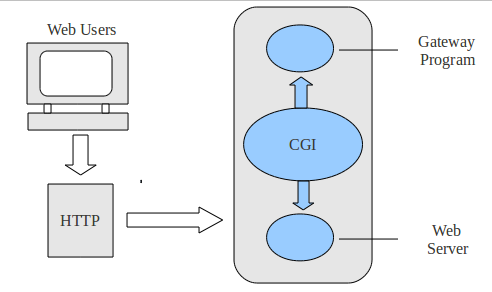
\includegraphics[width=1\textwidth]{figures/CGI.png}}
	\caption{CGI}
	\label{CGI}
\end{figure}
Common Gateway Interface atau disingkat CGI merupakan standar untuk menghubungkan berbagai program aplikasi ke halaman web. CGI mirip dengan program komputer yang menjadi perantara antara standar HTML yang menjadikan tampilan web dengan program lain, seperti basis data (database). Hasil yang diperoleh dari proses pencarian dikirimkan kembali ke halaman web untuk ditampilkan dalam format HTML.  \par
	\vspace{12pt}
CGI (Common Gateway Interface) adalah bentuk dari hubungan interaktif di mana client (browser) bisa mengirimkan suatu masukan kepada server, dan server mengolah masukan tersebut serta mengembalikannya kepada client (browser). Contoh sederhana adalah saat kita menggunakan sebuah mesin pencari. Saat kita menuliskan keyword dan menekan tombol Search maka browser akan mengirimkan keyword tersebut ke server. Keyword tersebut lalu diolah oleh server dan server mengirimkan data hasil pengolahan (yang sesuai dengan keyword yang kita masukkan) ke browser kita. Jadi yang akan kita lihat pada browser adalah  hanya data yang sesuai dengan keyword yang kita masukkan. \par
	
\subsection{Penggunaan CGI}
Untuk dapat menggunakan CGI syarat yang utama adalah server dengan sistem operasi UNIX (beserta variantnya). Namun perlu kita perhatikan bahwa tidak semua server UNIX (gratis) mampu menangani dan melayani CGI. Server-server yang melayani penempatan web yang berlayanan gratis seperti Geocities dan Homepage, tidak akan mengijinkan penggunaan script CGI dalam web kita. Untuk itu kita bisa mencoba Virtual Avenue, Tripod, atau Hypermart. \par
	\vspace{12pt}
	\noindent
	Program CGI ditulis dengan menggunakan bahasa yang dapat dimengerti oleh sistem misalnya C/C++, Fortran, Perl, Tcl, Visual Basic, dan lain-lain. Pemilihan bahasa yang digunakan tergantung dari sistem yang digunakan. Jika bahasa pemrograman yang digunakan seperti C atau Fortran maka program-program yang kita buat harus dikompile terlebih dahulu sebelum dijalankan sehingga pada server akan terdapat source code dan program hasil kompilasi. Berbeda jika bahasa yang digunakan yaitu bahasa script seperti PERL, TCL, atau Unix Shell maka hanya akan terdapat script itu sendiri (tanpa ada source code). Jika dibandingkan saat ini banyak orang yang lebih memilih untuk menggunakan script CGI daripada menggunakan bahasa pemrograman karena lebih mudah untuk di-compile dan dimodifikasi.  \par
	\vspace{12pt}
	\noindent
	Pada awalnya CGI merupakan~salah satu yang mendekati aplikasi server-side programming.  Program CGI yang paling sering digunakan yaitu~C++ dan perl.  CGI merupakan bagian dari web server yang dapat berkomunikasi dengan program lain yang ada di server. Dengan CGI web server dapat memanggil program yang dibuat dari berbagai bahasa pemrograman (Common). Interaksi antara pengguna dengan berbagai aplikasi, misalnya database, dapat dijembatani oleh CGI (Gateway). \par
	\vspace{12pt}
	\noindent
	CGI (Common Gateway Interface) merupakan skrip tertua dalam bidang pemrograman web. Skrip bisa didefinisikan sebagai rangkaian dari beberapa instruksi program. Untuk membuat skrip yang dapat dijalankan pada web diperlukan pengetahuan pemograman. \par
	\vspace{12pt}
	\noindent
	CGI sendiri telah muncul sejak teknologi web diperkenalkan di dunia pada awal tahun 1990, bersama dengan kemunculan CERN, web server pertama di dunia. CGI disediakan sebagai tool atau perlengkapan untuk membuat program web. CGI digunakan untuk membuat program-program tampilan web yang lebih interaktif, koneksi ke basis data, bahkan membuat permainan (game). \par
	\vspace{12pt}
	\noindent
	CGI pada masa-masa awalnya dibuat dengan bahasa C, bahasa yang juga digunakan untuk membuat web server pertama yaitu, CERN. CGI kemudian diadopsi oleh NCSA (National Central for Supercomputing Application) web server, dan hingga kini masih digunakan pada Apache Web Server, web server yang paling banyak digunakan oleh komunitas internet saat ini. \par
	\vspace{12pt}
	\noindent
	Walaupun demikian CGI bisa juga direalisasikan dengan banyak bahasa pemrograman lain. Mulai dari C, Perl, Phyton, PHP, Tcl/Tk, hingga skrip shell pada UNIX/LINUX. \par
	\vspace{12pt}
	\noindent
	CGI seringkali digunakan sebagai mekanisme untuk mendapatkan informasi dari user melalui fill out form, mengakses basis data (database), atau menghasilkan halaman yang dinamis. meskipun secara prinsip mekanisme CGI tidak memiliki lubang keamana, program atau skrip yang dibuat sebagai CGI dapat memiliki lubang keamanan ataupun tidak sengaja). Potensi lubang keamanan yang digunakan dapat terjadi dengan CGI antara lain : \par
	\noindent 
	\hspace*{0,5in}Seorang pemakai yang nakal dapat memasang skrip CGI sehingga dapat mengirimkan berkas kata kunci (password) kepada pengunjung yang mengeksekusi CGI tersebut. \par
		\noindent 
Program CGI dipanggil berkali-kali sehingga server menjadi terbebani karena harus menjalankan beberapa program CGI yang menghabiskan memori dan CPU cycle dari web server.
	\par
	\vspace{12pt}
	Sebuah aplikasi web berkomunikasi dengan perangkat lunak client melalui HTTP. HTTP, sebagai protokol yang berbicara menggunakan request dan response menjadikan aplikasi web bergantung kepada siklus ini untuk menghasilkan dokumen yang ingin diakses oleh pengguna. Secara umum, aplikasi web yang akan kita kembangkan harus memiliki satu cara untuk membaca HTTP Request dan mengembalikan HTTP Response ke pengguna. \par
	\vspace{12pt}
	Pada pengembangan web tradisional, kita umumnya menggunakan sebuah web server seperti Apache HTTPD atau nginx sebagai penyalur konten statis seperti HTML, CSS, Javascript, maupun gambar. Untuk menambahkan aplikasi web kita kemudian menggunakan penghubung antar web server dengan program yang dikenal dengan nama CGI (Common Gateway Interface). \par
	\vspace{12pt}
	CGI diimplementasikan pada web server sebagai antarmuka penghubung antara web server dengan program yang akan menghasilkan konten secara dinamis. Program-program CGI biasanya dikembangkan dalam bentuk script, meskipun dapat saja dikembangkan dalam bahasa apapun. Contoh dari bahasa pemrograman dan program yang hidup di dalam CGI adalah PHP. \par
	\noindent 
	Untuk melihat dengan lebih jelas cara kerja CGI, perhatikan penjelasan berikut: \par
	\noindent 
\hspace*{0,5in}item Web Server yang berhadapan langsung dengan pengguna, menerima HTTP Request dan mengembalikan HTTP Response. \par
		\noindent 
item Untuk konten statis seperti CSS, Javascript, gambar, maupun HTML web server dapat langsung menyajikannya sebagai HTTP Response kepada pengguna. Konten dinamis seperti program PHP maupun Perl disajikan melalui CGI. CGI Script kemudian menghasilkan HTML atau konten statis lainnya yang akan disajikan sebagai HTTP Response kepada pengguna.
	\par
	\vspace{12pt}
Meskipun terdapat banyak pengembangan selanjutnya dari CGI, ilustrasi sederhana di atas merupakan konsep inti ketika awal pengembangan CGI. Umumnya aplikasi web dengan CGI memiliki kelemahan di mana menjalankan script CGI mengharuskan web server untuk membuat sebuah proses baru. Pembuatan proses baru biasanya akan menggunakan banyak waktu dan memori dibandingkan dengan eksekusi script, dan karena setiap pengguna yang terkoneksi akan mengakibatkan hal ini terhadap server performa aplikasi akan menjadi kurang baik. \par
CGI sendiri menyediakan solusi untuk hal tersebut, misalnya FastCGI yang menjalankan aplikasi sebagai bagian dari web server. Bahasa lain juga menyediakan alternatif dari CGI, misalnya Java yang memiliki Servlet. Servlet pada Java merupakan sebuah program yang menambahkan fitur dari server secara langsung. Jadi pada pemrograman dengan Servlet, kita akan memiliki satu web server di dalam program kita, dan pada web server tersebut akan ditambahkan fitur-fitur spesifik aplikasi web kita. \par
	\vspace{12pt}
\textbf{KELEBIHAN CGI} \par
\noindent 
Kelebihan yang dimiliki CGI antara lain :  \par
\noindent 
\begin{enumerate}
	\item Skrip CGI dapat ditulis dalam bahasa apa saja, namun barangkali sekitar 90 $  \%  $ program CGI yang ada di tulis dalam Perl 
	\item Protokol CGI yang sederhana
	\item Kefasihan Perl dalam mengolah teks, menjadikan menulis sebuah program CGI cukup mudah dan cepat.
	\item Meski tertua hingga saat ini menurut survey dari Netcraft sekitar 70 $  \%  $ aplikasi di web masih menggunakan CGI. Ini berarti, lebih dari separuh situs Web dinamik yang ada dibangun dengan CGI.\end{enumerate}
\par
\vspace{12pt}
\noindent 
\textbf{KELEMAHAN CGI} \par
Salah satu kelemahannya ialah kecepatan yang rendah. Untuk menghasilkan keluaran program CGI, overhead yang harus ditempuh cukup besar, Dalam kasus CGI Perl, prosesnya sebagai berikut : \par
\noindent 
\begin{enumerate}
	\item Web server terlebih dahulu akan menciptakan sebuah proses baru dan menjalankan interpreter Perl.
	\item Perl kemudian mengkompilasi script CGI tersebut, baru kemudian menjalankan skrip.\end{enumerate}
\par
\vspace{12pt}
Keseluruhan siklus ini terjadi untuk setiap request. Dengan kata lain, terlalu banyak waktu yang dibuang untuk menciptakan proses dan tidak ada cache skrip yang telah dikompilasi. \par
\vspace{12pt}
Namun demikian, mungkin ini tidak lagi menjadi kendala di saat teknologi hardware untuk server sudah sedemikian maju; kecepata prosesor saat ini sudah cukup tinggi. Jika situs web menerima kurang dari sepuluh hingga dua puluh ribu hit CGI per hari, rata-rata mesin web server UNIX yang ada sekarang ini mampu menanganinya dengan baik. \par
\vspace{12pt}
\vspace{12pt}
\vspace{12pt}
\vspace{12pt}
\noindent 
Dalam kasus CGI Perl, prosesnya sbb: \par
\noindent 
\begin{itemize}
	\item Web server terlebih dahulu akan menciptakan sebuah proses baru dan menjalankan interpreter Perl.  \par
	\noindent 
	\item Perl kemudian mengkompilasi script CGI tersebut, baru kemudian menjalankan skrip.\end{itemize}
\par
\noindent 
Keseluruhan siklus ini terjadi untuk setiap request. Dengan kata lain, terlalu banyak waktu dibuang untuk menciptakan proses dan tidak ada cache skrip yang telah dikompilasi. \par
\noindent 
Jika sebuah situs web menerima kurang dari sepuluh hingga dua puluh ribu hit CGI per hari, rata-rata mesin web server Unix yang ada sekarang ini mampu menanganinya dengan baik. \par
\noindent 
Angka ini relatif, bergantung pada: \par
\noindent 
\begin{itemize}
	\item Tingkat pembebanan mesin web server untuk melakukan pekerjaan lain (misalnya, mengirim mail dan menjalankan server database) \par
	\noindent 
	\item Aplikasi CGI itu sendiri (sebab beberapa aplikasi CGI berupa skrip tunggal berukuran besar hingga waktu loading-nya cukup lama; umumnya aplikasi CGI yang rumit memecah diri menjadi skrip-skrip terpisah untuk mengurangi waktu loading). \par
	\noindent 
	\item Cepat atau lambatnya penampilan halaman web yang diterima klien akan lebih bergantung pada koneksi jaringan.\end{itemize}
\par
\vspace{12pt}
\noindent 
\textbf{Penerapan CGI} \par
Penerapan CGI yang paling umum adalah dalam pemrosesan . Umumnya, form dipergunakan untuk dua kegunaan~~~utama~.~ Yang  sederhana  adalah~~form~~yang  dipakai  untuk mengumpulkan informasi dari pengguna dan mengirimkanya~ke server. Namun  form~juga bisa dipakai untuk keperluan  yang~~lebih~ "canggih"  seperti timbal balik antara pengguna dan~server,~misalnya  form  yang memberikan sedaftar pilihan dokumen dalam~server kepada pengguna  untuk dipilih. Program CGI di server dibuat untuk~mengolah informasi ini  dan kemudian~~mengirimkan  dokumen - dokumen~~yang~~sesuai  dengan  pilihan pengguna. \par
\vspace{12pt}
Contoh nyata penerapan CGI untuk dokumen~~dinamis~~ini  misalnya  suatu "buku tamu". Pengguna memasukkan informasi seperti nama, alamat, alamat e-mail, dan komentar-komentarnya ke dalam form. Setelah server menerima informasi-informasi tadi, program CGI dapat~menyimpanya ke dalam  suatu File atau secara otomatis mengirimkanya lewat~e-mail~ke  suatu  alamat. Program~CGI~juga~bisa menampilkan dokumen yang  berisi  informasi  yang \par
\noindent 
baru~saja~dikirimkan~ oleh  pengguna  tadi~~sembari~~memberikan  ucapan  terima kasih atas partisipasinya. \par
\vspace{12pt}
Penerapan lain dari CGI adalah sebuah gateway.~Artinya~ adalah  program yang~dipergunakan sebagai penghubung  untuk~~mengakses~ informasi  yang tidak dapat secara langsung dibaca oleh program browser pengguna.Contoh yang nyata adalah gateway yang menghubungkan~antara~web  server  dengan dengan suatu database server yang besar semacam~oracle~~atau  DB2, yang  memang dapat dilakukan dengan mempergunakan bahasa pemrograman Perl dan DBI extentionta sehingga web server bisa~~memberikan~~query  dalam  SQL (structured query language, yaitu bahasa~yang~dipakai  untuk  melakukan pendefinisian maupun manipulasi terhadap~database)~ke  server  database Oracle. Setelah informasi dari database keluar, program CGI mengubahnya ke~dalam~bentuk~yang~bisa dibaca browser (HTML)  dan  web  server  pada giliranya mengirimkanya kepada browser. \par
\vspace{12pt}
Program CGI pada prinsipnya bisa ditulis~dalam~bahasa  pemrograman  apa saja,~namun~kenyataanya tidak  semua  bahasa~~pemrograman~ cocok  untuk pemrograman CGI. Penerapan CGI dapat sangat~kompleks, dan untuk membuat  suatu program CGI menuntut pengetahuan teknis~yang~~cukup  tinggi  akan pemrograman. \par
\vspace{12pt}
\vspace{12pt}
\noindent 
\textbf{Keamanan pada CGI} \par
CGI dapat menimbulkan lubang keamanan, karena program CGI dapat dijalankan di server lokal dari luar sistem (remote) oleh siapa saja. Apabila program CGI tidak didisain dan dikonfigurasi dengan baik, maka akan terjadi lubang keamanan. Kesalahan yang dapat terjadi antara lain: \par
\noindent 
\begin{itemize}
	\item program CGI mengakses berkas (file) yang seharusnya tidak boleh di akses. Misalnya pernah terjadi kesalahan dalam program phf sehingga digunakan oleh orang untuk mengakses berkas password dari server WW. \par
	\noindent 
	\item runaway CGI-script, yaitu program berjalan di luar kontrol sehingga mengabiskan CPU cycle dari server WWW\end{itemize}
\par
\vspace{12pt}
\noindent 
\textbf{Lubang Keamanan CGI} \par
\noindent 
Beberapa contoh lubang keamanan pada CGI \par
\noindent 
\begin{itemize}
	\item CGI dipasang oleh orang yang tidak berhak \par
	\noindent 
	\item CGI dijalankan berulang-ulang untuk menghabiskan resources (CPU, disk): DoS \par
	\noindent 
	\item Masalah setuid CGI di sistem UNIX, dimana CGI dijalankan oleh userid web server \par
	\noindent 
	\item Penyisipan karakter khusus untuk shell expansion \par
	\noindent 
	\item Kelemahan ASP di sistem Windows \par
	\noindent 
	\item Guestbook abuse dengan informasi sampah (pornografi) \par
	\noindent 
	\item Akses ke database melalui perintah SQL (SQL injection).\end{itemize}
\par
\vspace{12pt}
\noindent 
\textbf{Web Programming }\textbf{Python} \par
Python adalah bahasa pemrograman dinamis yang mendukung pemrograman berorientasi obyek. Python dapat digunakan untuk berbagai keperluan pengembangan perangkat lunak dan dapat berjalan di berbagai platform sistem operasi. Seperti halnya bahasa pemrograman dinamis, python seringkali digunakan sebagai bahasa skrip dengan interpreter yang teintergrasi dalam sistem operasi.

\begin{table}[ht]
	\caption{Sistem Basis Kode Python}
	\centering
	\begin{tabular}{cccc}
		\hline
		No&Sistem Operasi&\\
		\hline
		.1&Linux / Unix&\\
		.2&Windows&\\
		.3&Mac OS X&\\
		.4&Java Virtual Machine&\\
		.5&OS/2&\\
		.6&Amiga&\\
		.7&Palm&\\
		.8&Symbian (untukproduk-produk Nokia)&\\
		\hline
	\end{tabular}
\end{table}

Python didistribusikan dengan beberapa lisensi yang berbeda dari beberapa versi. Lihat sejarahnya di Python Copyright. Namun pada prinsipnya Python dapat diperoleh dan dipergunakan secara bebas, bahkan untuk kepentingan komersial. Lisensi Python tidak bertentangan baik menurut definisi Open Source maupun General Public License (GPL).
Python merupakan bahasa pemrograman yang mendukung pengembangan aplikasi berbasis desktop dan juga aplikasi berbasis web. Biasanya kalau berhubungan dengan WEB maka orang akan berfikir framework yang digunakan. Tentunya ada beberapa framework yang bisa digunakan untuk membangun aplikasi web berbasis python ini antara lain adalah Django, Web2py, Cherrypy dan lain-lain. Masing-masing framework memiliki aturan khusus dalam penulisan syntax. Framework tersebut mengadopsi struktur yang sama seperti pemrograman CGI. Untuk lebih jelasnya mari kita pelajari pemrograman CGI. 
Common Gateway Interface atau disingkat CGI adalah suatu standar untuk menghubungkan berbagai program aplikasi ke halaman web. CGI mirip sebuah program komputer yang menjadi perantara antara standar HTML yang menjadikan tampilan web dengan program lain, seperti basis data (database). Hasil yang diperoleh dari proses pencarian dikirimkan kembali ke halaman web untuk ditampilkan dalam format HTML. \par
\vspace{12pt}
Python menyediakan modul CGI yang bisa digunakan untuk membuat aplikasi berbasis web. Tentunya python tidak kalah dengan pemrograman berbasis web lain seperti Java, PHP dan lain2. Mari kita lakukan percobaan untuk membuat web dengan menggunakan python. \par
\noindent 
Hal Yang paling utama sebelum membuat aplikasi adalah mempersiapkan beberapa komponen aplikasi diantaranya adalah : \par
\noindent 
\begin{enumerate}
	\item Menginstal Program Python \par
	\noindent 
	\item Menginstal Program Web Server Seperti Apache2 atau Xampp \par
	\noindent 
	\item Setelah kedua program berhasil di instal maka langkah selanjutnya adalah mengkonfigurasi file httpd.conf yang berada pada directory web server, pada kesempatan ini saya menggunakan Xampp. \par
	\noindent 
	\item Buka directory Xampp dan masuk ke folder apache  $  \rightarrow  $ Conf dan cari file httpd.conf \par
	\noindent 
	\item Buka file httpd.conf menggunakan notepad \par
	\noindent 
	\item Cari baris AddHandler cgi-script .cgi .pl .asp pada file setelah itu tambahkan extensi python seperti ini AddHandler cgi-script .cgi .pl .asp .py \par
	\noindent 
	\item Cari baris <Directory /> dan tambahkan ExecCGI pada list Options FollowSymLinks \par
	\noindent 
	\item Setelah itu simpan \par
	\noindent 
	\item Selanjutnya kita akan mencoba membuat halaman web dasar pada python’ \par
	\noindent 
	\item Buka Notepad dan ketikkan script dbawah ini : \par
	\vspace{12pt}
	\noindent 
	\begin{verbatim}
	$  \#  $!/Python27/python
	print "Content-type:text/html" 
	print 
	print '<html>' 
	print '<head>' 
	print '<title>WEB Python </title>' 
	print '</head>' 
	print '<body>'
	print '<h1><center>Tutorial Web Programming Python Bagian 1 Python</center></h1>' 
	print 
	print
	print '<h2><center>Selamat Belajar Bagi Para Pecinta Python</h2></center>' \par
	\noindent 
	print '</body>' 
	print '</html>'
	\end{verbatim}
	pada script diatas jangan lupa menuliskan posisi directory python.exe ( $  \#  $!/Python27/python) \par
	\noindent 
	setelah itu simpan pada directory xampp folder cgi-bin dengan nama web.py (terserah nama apa saja asalhkan ekstensinya .py) \par
	\noindent 
	\item Buka browser dan ketikkan localhost/cgi-bin/web.py pada url dan lihatlah hasilnya\end{enumerate}
\par
\vspace{12pt}
\noindent 
\textbf{Membuat Kamus Menggunakan CGI Python} \par
Pertama yang kita butuhkan adalah sebuah kosa kata yang akan digunakan sebagai database, kosa kata tersebut kita convert kedalam format JSON. Untuk prosesnya sebagai berikut. Buatlah sebuah kosa kata bahasa indonesia dan bahasa inggris pada excel dengan header inggris dan indonesia. \par
\vspace{12pt}
Jika~sudah save as kedalam format .csv lalu di convert ke dalam format .json proses convert  bisa dilakukan secara online disini dan hasilnya akan seperti berikut dan simpan dengan nama kamus.json  \par
\vspace{12pt}
\noindent 
Selanjutnya kita mulai membuat script, buat sebuah file pada folder cgi-bin diserver localhost, tutorial ini menggunakan OS linux, ketikan script berikut. \par
\noindent 

$  \#  $!/usr/bin/python \par
\noindent 
\begin{equation}
import cgi
\end{equation}
import~cgitb; cgitb.enable()   \par
\noindent 
import simplejson as json \par
\vspace{12pt}
\noindent 
print "Content-type: text/html" \par
\noindent 
print \par
\vspace{12pt}
\noindent 
print """ \par
\noindent 
<html> \par
\noindent 
<head><title>CGI Script</title></head> \par
\noindent 
<body> \par
\noindent 
~ <h1> Kamus sederhana dengan cgi python</h1> \par
\noindent 
~ <form method="post" action="index.cgi"> \par
\noindent 
~~~ Bahasa Indonesia<br/> \par
\noindent 

~~~ <input type="text" name="kata"/></p> \par
\noindent 
~~~ <input type="submit" name="submit" value="Terjemahkan"/></p> \par
\noindent 
~ </form> \par
\noindent 
~~Bahasa Inggris<br/>   \par
\noindent 
""" \par
\vspace{12pt}
\noindent 
form = cgi.FieldStorage()  $  \#  $variable form \par
\noindent 
cari $  \_  $kata = form.getvalue("kata")  $  \#  $variable mengambil nilai dari input \par
\vspace{12pt}
\noindent 
location $  \_  $database = open('/home/develop/DW/kamus.json', 'r')  $  \#  $membuka kosa kata bahasa inggris \par
\noindent 
bhs $  \_  $inggris = json.load(location $  \_  $database) \par
\vspace{12pt}
\noindent 
if~cari $  \_  $kata:~   \par
\noindent 
~~ for bhs $  \_  $indonesia in cari $  \_  $kata.split(' '):  \par
\noindent 
~~~~for~arti $  \_  $kata in bhs $  \_  $inggris:    \par
\noindent 
~~~~ if arti $  \_  $kata["indonesia"] == bhs $  \_  $indonesia.replace(' ',''): \par
\noindent 
~~~~~~~~ hasil = arti $  \_  $kata['inggris']  \par
\noindent 
~~~~~~~ break \par
\noindent 
~~~ else: \par
\noindent 
~~~~~~~~hasil~= "arti kata tidak ditemukan"    \par
\noindent 
~~~~~~~~~~~~~~  \par
\noindent 
~~~ print """ \par
\noindent 
~~~ <input type="text" name="hasil" value=" $  \%  $s"/> \par
\noindent 
~~~ </body> \par
\noindent 
~~~ </html> \par
\noindent 
~~~ """  $  \%  $ cgi.escape(hasil) \par
\vspace{12pt}
Jika sudah save dengan nama kamus.cgi sebagai contoh dan buka browser ketikan pada url http//localhost/cgi-bin/kamus.cgi jika muncul form input coba di tester ketikan nama kata dalam bahasa indonesia. \par